\scanpage{26}
% archive sheet number: 25
\mspage{- 11 -}\hfill n$^{\mathrm{o}}$ 276

\figure{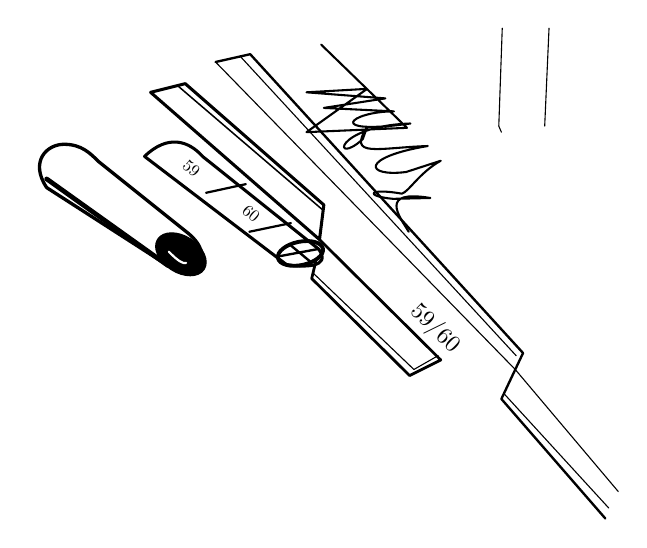
\begin{tikzpicture}[x=.11cm,y=.11cm,line cap=round,line join=round]
\draw[line width=1.2pt] (0,30) .. controls (-2,33) and (0,35) .. (2,35) .. controls (4,35) and (5,34) .. (6,33) -- (16,25) .. controls (20,22) and (17,19) .. (14,21) -- cycle;
\draw[line width=1.7pt] (0,31) -- (14,21);
\filldraw[rotate around={-33:(15.5,22.3)}] (15.5,22.3) ellipse (3.2 and 2.1);
\draw[white,line width=.8pt] (14.1,22.6) .. controls (15.2,21.5) and (15.7,21.2) .. (16.1,21.3);
\draw[line width=1.1pt] (12,41) -- (16,42) -- (32,28) -- (31.5,24) -- cycle;
\draw[line width=.55pt] (15.2,41.7) -- (31.9,27.4);
\draw[line width=1.1pt] (11.3,33.6) .. controls (14,36.2) and (16.4,35.4) .. (18,33.6) -- (31.4,22.9) .. controls (33,20.7) and (29.5,20.8) .. (27.7,21.1) -- cycle;
\draw[line width=.8pt] (18.4,29.4) -- (23,30.4) (23.4,24.9) -- (28.2,25.9);
\node[rotate=-40,scale=.61] at (16.7,32.2) {\handwritten{59}};
\node[rotate=-40,scale=.61] at (23.6,27.0) {\handwritten{60}};
\draw[line width=1.4pt,rotate around={12:(29.3,22.4)}] (29.3,22.4) ellipse (2.65 and 1.35);
\draw[line width=.85pt] (27,22.1) -- (31.3,22.9) (28.1,23.4) -- (30.5,21.4);
\draw[line width=1pt] (31.5,24) -- (45.5,10.1) -- (41.9,8.3) -- (30.6,19.5) -- (31.1,21.6);
\draw (30.8,20.1) -- (42.4,9.0) -- (45.2,10.6);
\draw[line width=.85pt] (19.5,44.5) -- (23.5,45.4) -- (55.0,10.9) -- (52.5,5.6) -- (64.5,-8.2);
\draw (22.4,45.1) -- (54.2,10.6) (19.5,44.5) -- (54.1,9.0) -- (66,-5.1) (52.9,6.1) -- (64.9,-7);
\node[rotate=-44,scale=.85] at (44.8,13.7) {\handwritten{59/60}};
\draw[line width=.75pt] (31.7,46.5) -- (41.6,36.9) -- (30,36.4) -- (37,41.4) -- (30,41) -- (39.1,40.3) -- (32,39.2) -- (40.1,38.8) .. controls (35,38.8) and (32,36) .. (42,37.4) .. controls (33,37.1) and (33,32.4) .. (36.5,35.6) -- (37,37) .. controls (34.7,33.4) and (38.2,34.6) .. (44,34.8) .. controls (36.2,33.5) and (36.7,31.2) .. (41.5,31.8) -- (45.5,33.1) .. controls (43,31.7) and (41.8,29.5) .. (41,29.3) .. controls (37,30) and (36.7,29.0) .. (40,28.7) -- (44.3,28.8) .. controls (38.3,29.8) and (40.7,26.7) .. (41.8,24.9);
\draw[thin] (52.6,48.4) -- (52.2,37.1) -- (52.5,36.4) (58,48.4) -- (57.5,37.1);
\end{tikzpicture}}

et par conséquent :
\[
a_n-\handwritten{\sum}_{i=\unsure{o|0}}^{i=i_p}a_{in}\handwritten{\in}\handwritten{\unsure{\mathfrak{m}|\mathrm{m}}}^{p-n}\quad.
\]

Considérant alors la série formelle $y=\handwritten{\sum} a_n X^n$, la relation précédente montre que l'on a
\[
y-\handwritten{\sum}_{i=o}^{i=i_p}y_i\handwritten{\in}\handwritten{\unsure{\mathfrak{n}|\mathrm{n}}}^p
\]
ce qui prouve que la série $\handwritten{\sum} y_i$ converge vers $y$, d'où la proposition.

\uline{Corollaire} - \uline{Soit} $A$ \uline{un anneau commutatif},. \uline{L'anneau de séries formelles} $A\handwritten{[[}X_1,\ldots,X_r\handwritten{]]}$ \uline{filtré par les puissances de l'idéal} $(X_1,\ldots X_r)$, \uline{est séparé et complet}.

5. - \uline{Modules de type fini sur un anneau filtré complet}.

Soient $(E,E_n)$ et $(F,F_n)$ deux modules filtrés sur un anneau filtré $(A,A_n)$ par un \uline{homomorphisme} $u:(E,E_n)\handwritten{\longrightarrow}(F,F_n)$ on entendra tout homomorphisme $u:E\handwritten{\longrightarrow} F$ de $A$-modules, tel que l'on ait
\[
u(E_n)\handwritten{\subset} F_n
\]
pour tout $n$. Si les filtrations de $E$ et $F$ sont associées à la filtration donnée de $A$, tout homomorph\deleted{\unsure{s|i}}isme de $A$-modules est un homomorphisme de modules filtrés\unsure{,|.}

Il est clair que tout homomorphisme $u:(E,E_n)\handwritten{\longrightarrow}(F,F_n)$ définit canoniquement un homomorphisme $G(u):G(E)\handwritten{\longrightarrow} G(F)$ des $G(A)$-modules gradués associés, obtenu par passage au quotient.

PROPOSITION 6 - \uline{Soient} $(E,E_n)$ \uline{et} $(F,F_n)$ \uline{deux modules filtrés sur un anneau filtré}, \uline{et} $u:(E,E_n)\handwritten{\longrightarrow}(F,F_n)$ \uline{un homomorphisme de modules filtrés}. \uline{Supposons remplies les conditions suivantes} :

a) : $(E,E_n)$ \uline{est complet}.

b) : $(F,F_n)$ \uline{est séparé}.

c) : \uline{l'homomorphisme associé} $G(u)$ \uline{est surjectif}\unsure{,|.}

